\documentclass[11pt,aspectratio=169]{beamer}

\usepackage{slides}
\usepackage{soul}
\usepackage{pdfpc}
\usepackage{ebproof}
\usepackage{bigdelim}
\usepackage{booktabs}
\usepackage{listings}
\usepackage{tcolorbox}
\usepackage{tabularx}
\usepackage{tikz}
\usepackage{xspace}
\usepackage[T1]{fontenc}
\usepackage[utf8]{inputenc}
\usepackage[symbol]{footmisc}
\usepackage[noend]{algpseudocode}
\usepackage[
    backend    = biber,
    style      = alphabetic,
    giveninits = true,
    maxnames   = 16,
    minnames   = 16,
]{biblatex}

\addbibresource{./references.bib}

\usetikzlibrary{
    positioning,
    shapes.symbols,
    shadows,
    arrows,
    calc
}

\newcommand{\senc}{\text{senc}}
\newcommand{\msg}{\text{msg}}
\newcommand{\nonce}{\text{nonce}}
\newcommand{\KDF}{\text{KDF}}
\newcommand{\key}{\text{key}}

\newcommand{\Tamarin}[1]{\textsc{Tamarin}\xspace}

%% Print: [#1] -[#2]-> [#3]
\newcommand{\MSR}[3]{#1 -\hspace{-4pt}[\hspace{5pt} #2 \hspace{4pt}]\hspace{-4.6pt}\rightarrow #3}
%% Print: -[#1]->
\newcommand{\ActionFact}[1]{-\hspace{-4pt}[\hspace{5pt} #1 \hspace{4pt}]\hspace{-4.6pt}\rightarrow}
%% Print: ~
\newcommand{\tildelow}{\raisebox{0.5ex}{\texttildelow}}
%% Print: ^
\newcommand{\pow}{\textasciicircum{}}
%% Highlight text in overlay
\newcommand{\althl}[2][2]{\alt<#1>{\hl{#2}}{#2}}

%% Sticky notes to represent facts
\definecolor{StickyNoteYellow}{RGB}{241,239,161}
\definecolor{StickyNoteRed}{RGB}{255,167,169}
\definecolor{StickyNoteGreen}{RGB}{148,199,146}
\definecolor{StickyNoteBlue}{RGB}{167,229,241}
\NewDocumentCommand{\StickyNote}{O{StickyNoteYellow}O{1cm}m}{%
    \begin{tikzpicture}
        \node[
            drop shadow={
                shadow xshift = 2pt,
                shadow yshift = -4pt,
            },
            xslant = -0.1,
            yslant = 0.1,
            draw   = black,
            fill   = #1,
            text   = black,
        ] {\parbox[t][#2][c]{#2}{\centering#3}};
    \end{tikzpicture}
}

%% Colors for terms and facts
\definecolor{TermBlue}{HTML}{1C377D}
\definecolor{FactPurple}{HTML}{7C3655}

\newcommand{\term}[1]{\textcolor{TermBlue}{#1}}
\newcommand{\Term}[1]{\textcolor{TermBlue}{#1}}
\newcommand{\Fact}[1]{\textcolor{FactPurple}{#1}}

%% Other colors
\definecolor{AdversaryRed}{HTML}{DA3B26}

%% Listings
\lstset{escapeinside={(*@}{@*)}}
\lstset{numberstyle=\tiny}

\definecolor{TamarinBlue}{RGB}{42,0,255}
\definecolor{TamarinGreen}{RGB}{48,110,32}
\definecolor{TamarinPurple}{RGB}{175,36,67}

\lstdefinestyle{tamarin}{
    basicstyle    = \linespread{0.75}\footnotesize\ttfamily,
    extendedchars = true,
    tabsize       = 2,
    columns       = fixed,
    numbers       = none,
    breaklines    = true,
    literate      = {~}{{\raisebox{0.5ex}{\texttildelow}}}{1},
    morekeywords  = {theory, builtins, restriction, equations, functions, rule,
                     let, in, lemma, All, Ex, not, predicates, begin, end},
    keywordstyle  = \color{TamarinPurple},
    morecomment   = [l]{//},
    morecomment   = [s]{/*}{*/},
    commentstyle  = \color{TamarinGreen},
    xleftmargin   = 0mm,
    upquote       = true,
    morestring    = *[b]",
    showstringspaces = false
}

\lstdefinestyle{tactic}{
    basicstyle    = \linespread{0.75}\footnotesize\ttfamily,
    extendedchars = true,
    tabsize       = 2,
    columns       = fixed,
    numbers       = none,
    breaklines    = true,
    literate      = {~}{{\raisebox{0.5ex}{\texttildelow}}}{1},
    alsoletter    = :,
    morekeywords  = {tactic:, presort:, prio:, deprio:},
    keywordstyle  = \color{TamarinPurple},
    morecomment   = [l]{//},
    morecomment   = [s]{/*}{*/},
    commentstyle  = \color{TamarinGreen},
    xleftmargin   = 0mm,
    upquote       = true,
    morestring    = *[b]",
}

\lstdefinestyle{oracle}{
    basicstyle    = \linespread{0.75}\footnotesize\ttfamily,
    extendedchars = true,
    tabsize       = 2,
    columns       = fixed,
    numbers       = none,
    breaklines    = true,
    literate      = {~}{{\raisebox{0.5ex}{\texttildelow}}}{1},
    morecomment   = [l]{\#},
    morekeywords  = {import, for, in, if, elif},
    keywordstyle  = \color{TamarinPurple},
    commentstyle  = \color{TamarinGreen},
    xleftmargin   = 0mm,
    upquote       = true,
}

\definecolor{ProVerifGreen}{RGB}{48,110,32}
\definecolor{ProVerifBlue}{RGB}{64,112,161}

\lstdefinestyle{proverif}{
    basicstyle    = \linespread{0.75}\footnotesize\ttfamily,
    extendedchars = true,
    tabsize       = 2,
    columns       = fixed,
    numbers       = none,
    breaklines    = true,
    literate      = {~}{{\raisebox{0.5ex}{\texttildelow}}}{1},
    morecomment   = [s]{(*}{*)},
    commentstyle  = \color{ProVerifGreen},
    keywordstyle  = \color{ProVerifBlue},
    morekeywords  = {in, if, event, new, let, out},
    xleftmargin   = 0mm,
}

\definecolor{proofTreeBlue}{HTML}{2639B0}
\definecolor{proofTreeRed}{HTML}{921C12}

\lstdefinestyle{prooftree}{
    basicstyle    = \linespread{0.8}\footnotesize\fontfamily{pcr}\selectfont,
    extendedchars = true,
    tabsize       = 2,
    columns       = fixed,
    numbers       = left,
    breaklines    = true,
    literate      = {~}{{\raisebox{0.5ex}{\texttildelow}}}{1},
    keywords      = [1]{lemma, case, next, qed, by, end, Diff-Lemmas},
    keywordstyle  = [1]\color{black}\bfseries,
    keywords      = [2]{simplify, solve, sorry, contradiction, induction,
                        autoprove, rule-equivalence},
    keywordstyle  = [2]\color{proofTreeBlue}\bfseries,
    keywords      = [3]{@, \|, <, \^},
    keywordstyle  = [3]\color{proofTreeRed},
    alsoletter    = @\|<\^-,
    moredelim     = **[is][{\color{proofTreeBlue}}]{<<}{>>},
    xleftmargin   = 0mm,
    upquote       = true,
    morestring    = *[b]",
}

%% Color boxes
\definecolor{ColorBoxBlue}{HTML}{1C377D}
\tcbset{
    colback      = white,
    colframe     = black,
    fonttitle    = \bfseries,
    coltitle     = white,
    colbacktitle = ColorBoxBlue,
    boxrule      = 1pt
}

%% Vertical separator for frames
\newcommand<>{\vsep}{
    \begin{tikzpicture}[remember picture,overlay]%
        \draw[ultra thick]
            ($(current page.north west)+(8cm,0.5cm)$) to
            ($(current page.south west)+(8cm,-0.5cm)$)
        ;
    \end{tikzpicture}%
}

%% Horizontal separator for frames
\newcommand<>{\hsep}{
    \begin{tikzpicture}[remember picture,overlay]%
        \draw[ultra thick]
            ($(current page.north west)+(-0.5cm,-4.5cm)$) to
            ($(current page.north east)+(0.5cm,-4.5cm)$)
        ;
    \end{tikzpicture}%
}


\title{Formal Analysis of Real-World Security Protocols}
\subtitle{Lecture 3: Attacker Model and Trace Properties}
\date{\today}
\author{Aleksi Peltonen}
\institute{CISPA Helmholtz Center for Information Security}

\begin{document}
\maketitle

% ---------------------------------------------------------------------------- %
% Content
% ---------------------------------------------------------------------------- %

\begin{frame}[fragile]{Model components}
    What \textbf{components} do we need to model protocols?

    \begin{table}
        \raggedright
        \begin{tabular}{lll}
            1. & All possible sent and received messages
               & \rdelim\}{1}{3mm}[\hspace*{3mm}Lecture 1] \\[.2cm]
            2. & All possible protocol behaviors
               & \rdelim\}{1}{3mm}[\hspace*{3mm}Lecture 2] \\[.2cm]
            3. & The attacker
               & \rdelim\}{2.2}{3mm}[\hspace*{2mm}\hl{Lecture 3}] \\[.2cm]
            4. & Security properties that we want to verify
        \end{tabular}
    \end{table}
\end{frame}

\begin{frame}[fragile]{This lecture}
    \tableofcontents
\end{frame}

% ---------------------------------------------------------------------------- %

\section{Actions and Action Traces}

% ---------------------------------------------------------------------------- %

\begin{frame}[fragile]{Action facts}
    \begin{itemize}
        \item \textbf{Actions}, like regular facts, are built from predicates 
              applied to terms
        \item They model actions taken by agents during protocol execution and 
              steps taken during protocol initialization
        \vspace*{.5cm}
        \begin{onlyenv}
            \begin{table}[]
                \hspace*{-10cm}
                \begin{tabular}{c}
                    \begin{lstlisting}[
                        style=tamarin,
                        gobble = 10,
                        escapechar = @,
                        basicstyle=\linespread{0.75}\ttfamily,
                    ]
                        // Send message
                        [ Fr(~m) ] @\textcolor{TamarinBlue}{ ---[ Send(\tildelow{}m) ]->}@ [ Out(~m) ]

                        // Receive message
                        [ In(m)  ] @\textcolor{TamarinBlue}{ ---[ Receive(m) ]->}@ [ ]
                    \end{lstlisting}
                \end{tabular}
            \end{table}
        \end{onlyenv}
        \item Actions are analogous to labels in labelled transition systems and can be used for \textbf{property specification}
    \end{itemize}
\end{frame}

\begin{frame}[fragile]{Executions}
    \begin{itemize}
        \item Let $R$ be a set of rules constructed over a given signature, and 
              let $S$ be a state of the system, i.e., a multiset of facts
        \item An \textbf{execution} of $R$ with respect to an equational theory 
              $E$ is an alternating sequence of states and ground rule 
              instances:
        \begin{center}
            [ $S_0, \MSR{l_1}{a_1}{r_1}$,
              $S_1, \MSR{l_2}{a_2}{r_2}$, $\dots$,
              $S_{k-1}, \MSR{l_k}{a_k}{r_k}$, $S_k$ ]
        \end{center}
        such that the following three conditions hold:
        \begin{enumerate}
            \item $S_0$ = [ ],
            \item $\forall i \in \{1 \dots k\}$, ($S_{i-1}, 
                  (\MSR{l_i}{a_i}{r_i}), S_i) \in steps(R)$, and
            \item $\forall i,j \in \{1 \dots k\}$,
                  $r_i = \MSR{[\;]}{}{[Fr(n)]}$ and
                  $r_j = \MSR{[\;]}{}{[Fr(n)]}$: $i=j$.
        \end{enumerate}
        \item We denote the set of executions of a set of rules $R$ by
              $execs(R)$
    \end{itemize}
\end{frame}

\begin{frame}[fragile]{Traces}
    \begin{itemize}
        \item For each execution, we define the corresponding trace as the 
              sequence $[set(a_1), set(a_2), \dots, set(a_k)]$ and denote the 
              set of all traces of a set of rules $R$ by $traces(R)$
        \item Consider the following protocol:\\[0.2cm]

        \begin{lstlisting}[style=tamarin, gobble=8]
            [      ] --[ Init()  ]-> [ A('1') ] // Create A('1')
            [ A(x) ] --[ Step(x) ]-> [ B(x)   ] // Convert A(x) to B(x)
        \end{lstlisting}

        \item One possible execution:\\[0.2cm]

        \begin{lstlisting}[style=tamarin, gobble=10]
            [                ] --[ Init()    ]->
            [ A('1')         ] --[ Init()    ]->
            [ A('1'), A('1') ] --[ Step('1') ]->
            [ A('1'), B('1') ]
        \end{lstlisting}

        \item Corresponding trace:\\[0.2cm]

        \begin{lstlisting}[style=tamarin, gobble=8]
            [ Init(), Init(), Step('1') ]
        \end{lstlisting}
    \end{itemize}
\end{frame}

% ---------------------------------------------------------------------------- %

\section*{Example}

% ---------------------------------------------------------------------------- %

\begin{frame}[fragile]{Needham-Schroeder Public-Key protocol (NSPK)}
    \begin{figure}
        \includegraphics<1>[width=.9\textwidth]
            {./figures/lecture_3/nspk}%
        \includegraphics<2>[width=.9\textwidth]
            {./figures/lecture_3/nspk_actions_1}%
        \includegraphics<3>[width=.9\textwidth]
            {./figures/lecture_3/nspk_actions_2}%
    \end{figure}
\end{frame}

\begin{frame}[fragile]{Protocol model}
    \begin{figure}
        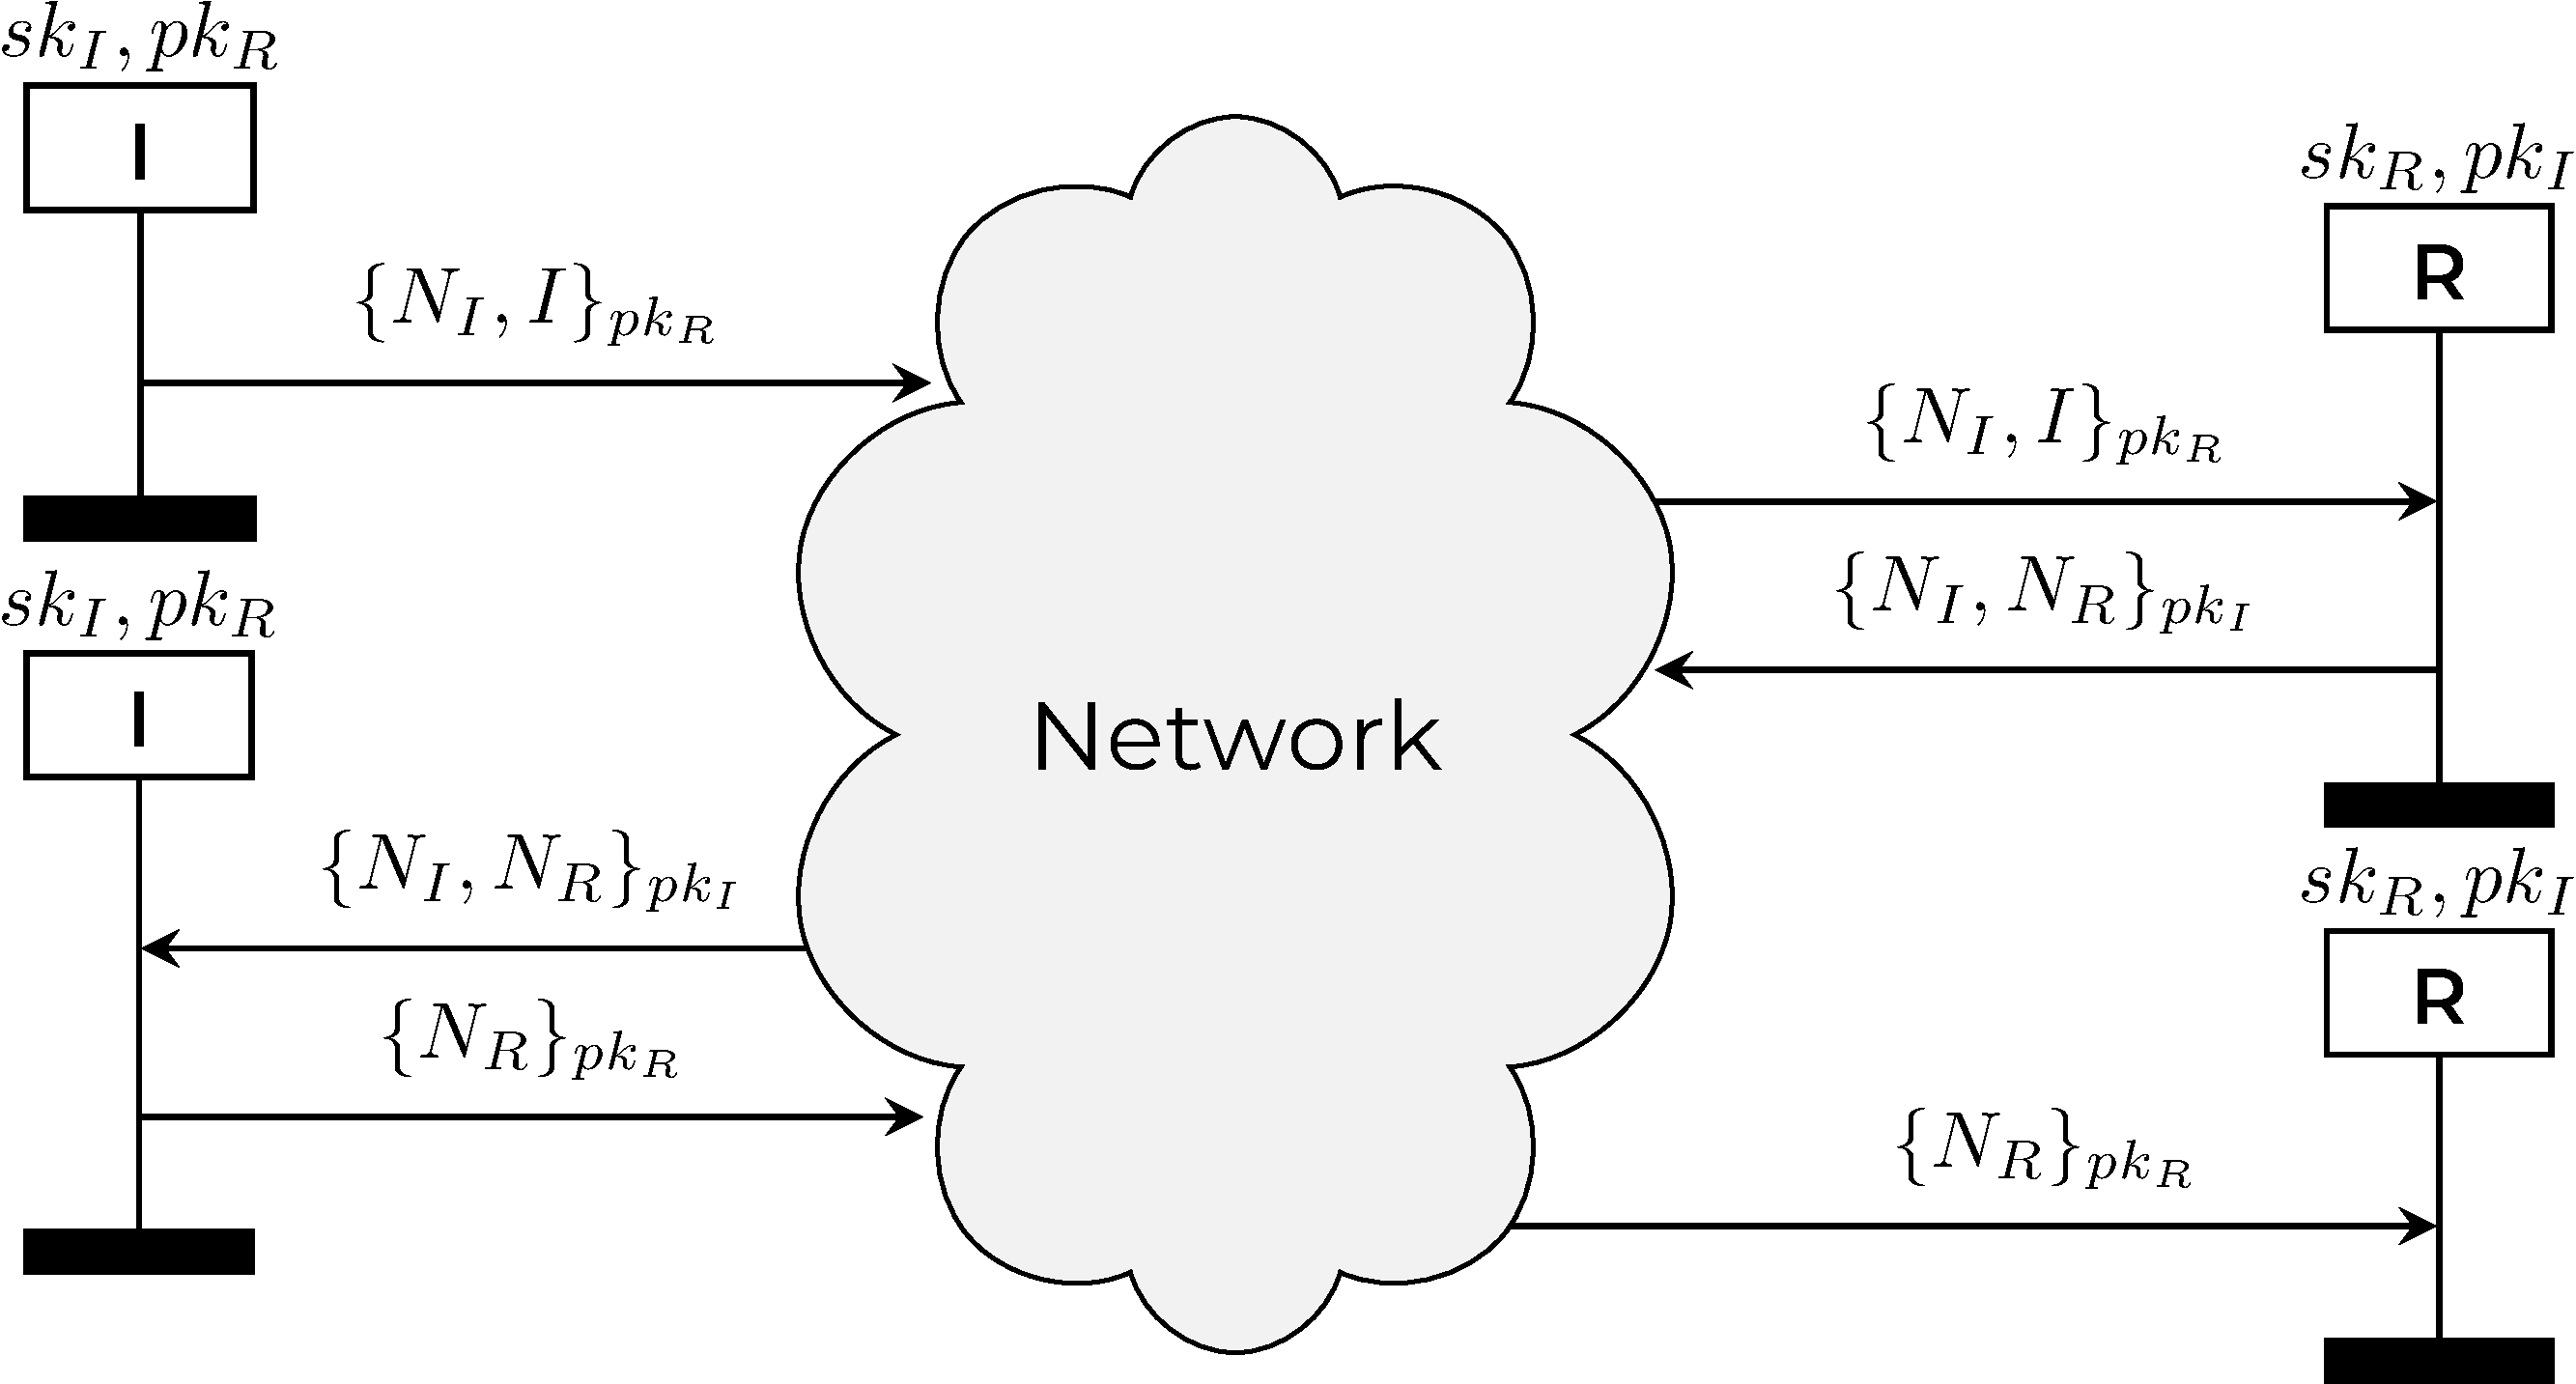
\includegraphics[width=.8\textwidth]{./figures/lecture_3/nspk_split_1}
    \end{figure}
\end{frame}

\begin{frame}[fragile]{Initialization}
    \begin{columns}
        \begin{column}{0.5\textwidth}
            \begin{figure}
                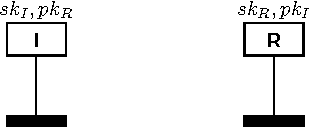
\includegraphics[width=.8\textwidth]
                    {./figures/lecture_3/nspk_init}
            \end{figure}
        \end{column}
        \begin{column}{0.5\textwidth}
            \begin{lstlisting}[style=tamarin, gobble=16]
                builtins: asymmetric-encryption


                /* Public key infrastructure */
                rule register_pk:
                    let
                      public_key = pk(~secret_key)
                    in
                    [ Fr(~secret_key) ]
                    -->
                    [ !Sk($ID, ~secret_key)
                    , !Pk($ID, public_key)
                    , Out(public_key) ]


                /* Reveal secret key */
                rule reveal_sk:
                    [ !Sk(ID, secret_key) ]
                  --[ Reveal(ID) ]->
                    [ Out(secret_key) ]
            \end{lstlisting}
        \end{column}
    \end{columns}
    \vsep
\end{frame}

\begin{frame}[fragile]{Initiator (1/2)}
    \begin{columns}
        \begin{column}{0.5\textwidth}
            \begin{figure}
                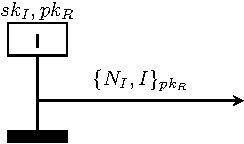
\includegraphics[width=.8\textwidth]
                    {./figures/lecture_3/nspk_i1}
            \end{figure}
        \end{column}
        \begin{column}{0.5\textwidth}
            \begin{lstlisting}[style=tamarin, gobble=16]
                /* Generate a fresh nonce nI and
                   send an encrypted message
                   to R. */
                rule initiator_1:
                    let
                      m1 = aenc{'1', ~nI, $I}pkR
                    in
                    [ Fr(~nI)
                    , !Pk($R, pkR) ]
                  --[ Send(m1) ]->
                    [ Out(m1)
                    , St_I_1($I, $R, ~nI) ]
            \end{lstlisting}
        \end{column}
    \end{columns}
    \vsep
\end{frame}

\begin{frame}[fragile]{Responder (1/2)}
    \begin{columns}
        \begin{column}{0.5\textwidth}
            \begin{figure}
                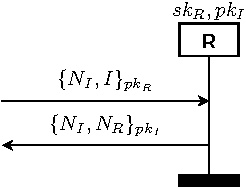
\includegraphics[width=.8\textwidth]
                    {./figures/lecture_3/nspk_r1}
            \end{figure}
        \end{column}
        \begin{column}{0.5\textwidth}
            \begin{lstlisting}[style=tamarin, gobble=16]
                /* Receive an encrypted message
                   from I and decrypt it.
                   Derive a fresh nonce nR and
                   reply to I. */
                rule responder_1:
                    let
                      m1 = aenc{'1', nI, I}pk(skR)
                      m2 = aenc{'2', nI, ~nR}pkI
                    in
                    [ In(m1)
                    , !Sk(R, skR)
                    , !Pk(I, pkI)
                    , Fr(~nR) ]
                  --[ Receive(nI, m1)
                    , Send(m2)
                    , Running(R, I, ~nR, nI) ]->
                    [ Out(m2)
                    , St_R_1(R, I, nI, ~nR) ]
            \end{lstlisting}
        \end{column}
    \end{columns}
    \vsep
\end{frame}

\begin{frame}[fragile]{Initiator (2/2)}
    \begin{columns}
        \begin{column}{0.5\textwidth}
            \begin{figure}
                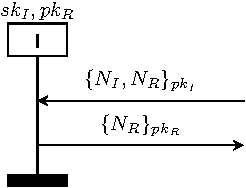
\includegraphics[width=.8\textwidth]
                    {./figures/lecture_3/nspk_i2}
            \end{figure}
        \end{column}
        \begin{column}{0.5\textwidth}
            \begin{lstlisting}[style=tamarin, gobble=16]
                /* Receive an encrypted message
                   from R and decrypt it.
                   Respond to R. */
                rule initiator_2:
                    let
                      m2 = aenc{'2', nI, nR}pk(skI)
                      m3 = aenc{'3', nR}pkR
                    in
                    [ In(m2)
                    , St_I_1(I, R, nI)
                    , !Sk(I, skI)
                    , !Pk(R, pkR) ]
                  --[ Receive(nR, m2)
                    , Running(I, R, nI, nR)
                    , Commit(I, R, nI, nR) ]->
                    [ Out(m3) ]
            \end{lstlisting}
        \end{column}
    \end{columns}
    \vsep
\end{frame}

\begin{frame}[fragile]{Responder (2/2)}
    \begin{columns}
        \begin{column}{0.5\textwidth}
            \begin{figure}
                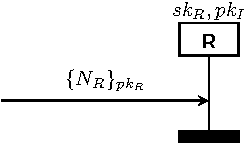
\includegraphics[width=.8\textwidth]
                    {./figures/lecture_3/nspk_r2}
            \end{figure}
        \end{column}
        \begin{column}{0.5\textwidth}
            \begin{lstlisting}[style=tamarin, gobble=16]
                /* Receive a message from I. */
                rule responder_2:
                    let
                      m3 = aenc{'3', nR}pk(skR)
                    in
                    [ In(m3)
                    , St_R_1(R, I, nI, nR)
                    , !Sk(R, skR) ]
                  --[ Commit(R, I, nR, nI) ]->
                    [  ]
            \end{lstlisting}
        \end{column}
    \end{columns}
    \vsep
\end{frame}

% ---------------------------------------------------------------------------- %

\section{Protocol Model}

% ---------------------------------------------------------------------------- %

\begin{frame}[fragile]{Protocol model in Tamarin}
    \begin{itemize}
        \item \textbf{Term algebra}
        \begin{itemize}
            \item $\Sigma_{DH} = \{enc(\_,\_),dec(\_,\_),h(\_),\langle\_,
                  \_\rangle,fst(\_),snd(\_), \_\hat{\;}\_ , \_^{-1}, 
                  \_\times\_, 1\}$
        \end{itemize}
        \item \textbf{Equational theory}
        \begin{itemize}
            \item $E_{DH} = \{dec(enc(m,k),k) =_E m$, $x \times (y \times z) 
                  =_E (x \times y) \times z$, $\dots \}$
        \end{itemize}
        \item \textbf{Facts}
        \begin{itemize}
            \item $F(t_1, \dots, t_n)$
        \end{itemize}
        \item \textbf{Transition system}
        \begin{itemize}
            \item State: multiset of facts
            \item Rules: $\MSR{l}{a}{r}$
        \end{itemize}
        \item \textbf{Special facts and rules}
        \begin{itemize}
            \item Facts: $In()$, $Out()$, $K()$
            \item Special fresh rule: $\MSR{[\;]}{}{[\;Fr(x)\;]}$
        \end{itemize}
    \end{itemize}
\end{frame}

\begin{frame}[fragile]{Semantics}
    \begin{itemize}
        \item \textbf{Transition relation}
        \begin{itemize}
            \item[] $S\,\ActionFact{a}_R\,(( S \smallsetminus^{\#} l )
                    \cup^{\#} r)$, where
            \begin{itemize}
                \item $\MSR{l}{a}{r}$ is a ground instance of 
                      a rule in $R$, and
                \item $l\subseteq^{\#}S$ wrt the equational theory
            \end{itemize}
        \end{itemize}
        \item \textbf{Executions}
        \begin{itemize}
            \item $execs(R) = \{\;[\;]\,\ActionFact{a_1} \dots \ActionFact{a_n}
                  \, S_n \;|\; \forall n .\; Fr(n)$
                  appears only once on the right-hand side of the rule\;\}
        \end{itemize}
        \item \textbf{Traces}
        \begin{itemize}
            \item $traces(R) = \{\; [a_1, \dots , a_n] \;|\; [\;]\,\ActionFact
                  {a_1} \dots \ActionFact{a_n}\, S_n \in execs(R)\;\}$
        \end{itemize}
    \end{itemize}
\end{frame}

% ---------------------------------------------------------------------------- %

\section{Attacker Model}

% ---------------------------------------------------------------------------- %

\begin{frame}[fragile]{Attacker model}
    Recall the \textbf{protocol execution model} from earlier:
    \begin{figure}
        \includegraphics<1>[width=.6\textwidth]
            {./figures/lecture_3/nspk_split_1}%
        \includegraphics<2>[width=.6\textwidth]
            {./figures/lecture_3/nspk_split_2}
    \end{figure}
\end{frame}

\begin{frame}[fragile]{The Dolev-Yao model}
    \begin{itemize}
        \item All messages are sent to the attacker who can either
              \textbf{drop}, \textbf{modify}, or \textbf{forward} them
        \item The attacker sees all the messages and maintains a knowledge set 
              of all the information sent over public channels
        \item When the attacker learns a cryptographic key, it can perform 
              cryptographic operations, such as \textbf{encryption},
              \textbf{decryption}, and \textbf{signing}, to add new messages to 
              its knowledge set
        \item The attacker can also deconstruct messages into their components 
              and create new messages from the parts it knows
        \item However, it cannot forge or read cryptographically protected 
              messages \textbf{without knowing the corresponding keys}
    \end{itemize}
\end{frame}

\begin{frame}[fragile]{Some potential attacks}
    \begin{itemize}
        \item[] \textbf{Man-in-the-middle:} $c$ impersonates $a$ to $b$
        \item[] \textbf{Replay:} reuse previous messages
        \item[] \textbf{Reflection:} send message back to its sender
        \item[] \textbf{Oracle:} use normal protocol responses to gain 
                                 information
        \item[] \textbf{Binding:} use messages in an unintended context
        \item[] \textbf{Type flaw:} substitute message fields
    \end{itemize}
\end{frame}

\begin{frame}[fragile]{Attacker knowledge and interaction}
    \begin{itemize}
        \item A persistent fact \textbf{K(m)} denotes that \textit{m} is known 
              to the adversary
        \item A linear fact \textbf{Out(m)} denotes that the protocol has sent 
              the message \textit{m}, which can be received by the adversary
        \item A linear fact \textbf{In(m)} denotes that the protocol can 
              receive the message \textit{m}, which might have been sent by the 
              attacker
        \item The semantics of these three fact symbols is given by the 
              following set of \textbf{message deduction rules}
    \end{itemize}
\end{frame}

\begin{frame}[fragile]{Message deduction rules}
    \begin{table}[]
        {\renewcommand{\arraystretch}{1.5}
        \begin{tabular}{rl}
            $\mathrm{\left\{\dfrac{Out(x)}{K(x)}\right\}}$ &
                \begin{lstlisting}[style=tamarin, gobble=20]
                    // Receive message from the protocol
                    [ Out(x) ] --> [ K(x) ]
                \end{lstlisting}\\[2mm]
            $\mathrm{\left\{\dfrac{K(x)}{In(x)}[K(x)]\right\}}$ &
                \begin{lstlisting}[style=tamarin, gobble=20]
                    // Send message to the protocol
                    [ K(x) ] --[ K(x) ]-> [ In(x) ]
                \end{lstlisting}\\[2mm]
            $\mathrm{\left\{\dfrac{}{K(x:pub)}\right\}}$ &
                \begin{lstlisting}[style=tamarin, gobble=20]
                    // Learn public value
                    [ ] --> [ K($x) ]
                \end{lstlisting}\\[2mm]
            $\mathrm{\left\{\dfrac{Fr(x:fresh)}{K(x:fresh)}\right\}}$ &
                \begin{lstlisting}[style=tamarin, gobble=20]
                    // Generate fresh value
                    [ Fr(~x) ] --> [ K(~x) ]
                \end{lstlisting}\\[2mm]
            $\mathrm{\left\{\dfrac{K(x_1)\dots
                     K(x_k)}{K(f(x_1\dots x_k))}\right\}}$ &
                \begin{lstlisting}[style=tamarin, gobble=20]
                    // Apply functions to known messages
                    [ K(x_1)...K(x_k) ] --> [ K(f(x_1...x_k)) ]
                \end{lstlisting}
        \end{tabular}}
    \end{table}
\end{frame}

% ---------------------------------------------------------------------------- %

\section{Trace Properties}

% ---------------------------------------------------------------------------- %

\begin{frame}[fragile]{Trace properties}
    \begin{itemize}
        \item A trace property specifies a set of traces representing a set of 
              desired protocol behaviors
        \item If the protocol state machine includes behaviors that are not 
              included in the specified property, then we have a violation
        \begin{itemize}
            \item[$\rightarrow$] \textbf{This constitutes an attack on the 
                                         protocol!}
        \end{itemize}
        \item In Tamarin, trace properties are specified as formulas in
              \textbf{first-order logic}, built from actions and quantifying 
              over message terms and timepoints
        \item Timepoints are are used to order actions; they enable the 
              specification of properties that depend on the events' relative 
              ordering
    \end{itemize}
\end{frame}

\begin{frame}[fragile]{Syntax}
    \begin{table}[]
        \begin{tabular}{ll}
            \texttt{All} & Universal quantification ($\forall$) \\
            \texttt{Ex}  & Existential quantification ($\exists$) \\
            \texttt{==>} & Implication \\
            \texttt{\&}  & Conjunction \\
            \texttt{|}   & Disjunction \\
            \texttt{not} & Negation ($\neg$) \\
            \texttt{f@i} & An action \texttt{f} at a timepoint \texttt{\#i} \\
            \texttt{\#i < \#j}
              & Timepoint \texttt{\#i} occurring before \texttt{\#j} \\
            \texttt{\#i = \#j} & Timepoint equality \\
            \texttt{x = y} & Message variable equality \\
            \texttt{Pred}($t_1, \dots, t_n$)
              & The predicate \texttt{Pred} applied to the terms $t_1$ to $t_n$
        \end{tabular}
    \end{table}
\end{frame}

% ---------------------------------------------------------------------------- %

\section*{Example}

% ---------------------------------------------------------------------------- %

\begin{frame}[fragile]{Needham-Schroeder Public-Key protocol (NSPK)}
    \begin{figure}
        \includegraphics<1>[width=.9\textwidth]
            {./figures/lecture_3/nspk}%
        \includegraphics<2>[width=.9\textwidth]
            {./figures/lecture_3/nspk_actions_2}%
    \end{figure}
\end{frame}

\begin{frame}[fragile]{Lemma 1: Executability}
    To rule out (some) modeling mistakes, we use reachability lemmas to make 
    sure that it is \textbf{possible} to reach the end of the protocol model. 
    Our goal is to find a completed protocol trace where the steps are the 
    expected ones taken by honest agents without adversary interference.
    \vfill
    \begin{center}
        \begin{tabular}{c}
            \begin{lstlisting}[style=tamarin, gobble=16]
                /* Executability */
                lemma trace: exists-trace
                    " Ex A B nA nB #i #j .
                        Commit(A, B, nA, nB)@i
                      & Commit(B, A, nB, nA)@j
                      & not(Ex #r. Reveal(A)@r)
                      & not(Ex #r. Reveal(B)@r)
                    "
            \end{lstlisting}
        \end{tabular}
    \end{center}
\end{frame}

\begin{frame}[fragile]{Lemma 2: Injective agreement}
    Whenever somebody commits to running a session and the adversary did not 
    reveal the long-term key of the participants, there is somebody running a 
    session with the same parameters and there is no other commit on the same 
    parameters.\vfill
    \begin{center}
        \begin{tabular}{c}
            \begin{lstlisting}[style=tamarin, gobble=16]
                /* Injective agreement */
                lemma injective_agreement:
                    " All A B nA nB #i .
                        Commit(A, B, nA, nB)@i
                        ==> (Ex #j. Running(B, A, nB, nA)@j & j < i
                             & not(Ex A2 B2 #i2 .
                                Commit(A2, B2, nA, nB)@i2 & not(#i = #i2)))
                          | (Ex #r. Reveal(A)@r)
                          | (Ex #r. Reveal(B)@r)
                    "
            \end{lstlisting}
        \end{tabular}
    \end{center}
\end{frame}

% ---------------------------------------------------------------------------- %

\section*{Summary}

% ---------------------------------------------------------------------------- %

\begin{frame}[fragile]{Summary}
    \begin{itemize}
        \item We now know how to model..
        \begin{itemize}
            \item ..protocol behavior as \textbf{multiset rewriting rules}
            \item ..protocol properties as \textbf{first-order logic formulas}
        \end{itemize}
        \item Together, these two languages allow us to
              \textbf{model protocols}, \textbf{specify security properties}, 
              and \textbf{analyze them in the presence of a Dolev-Yao attacker}
        \item In the next lecture, we will talk about how Tamarin uses this 
              model to find attacks
    \end{itemize}
\end{frame}

% ---------------------------------------------------------------------------- %
% Reading Material
% ---------------------------------------------------------------------------- %
\begin{frame}[fragile]{Reading material}
    \textbf{Recommended reading}: \\ \;
        ~\cite[Ch. 3.2.2, 4, 5--5.8]{tamarin-book},
        ~\cite[Ch. 7.3]{meier2013thesis},
        ~\cite{schmidt2012tamarin}
    \printbibliography[heading=none]
\end{frame}
% ---------------------------------------------------------------------------- %

\end{document}
